\chapter{A radiação de Cherenkov}\label{apdx:cherenkov}

Techniques for nuclear and particle physics experiments, a how-to approach - W.R. Leo

A radiação de Cherenkov acontece quando partículas carregadas atravessando um meio têm velocidades maiores que a velocidade da luz naquele meio, ou seja:

\begin{equation}
    v_{partícula} > \dfrac{c}{n}
\end{equation}

onde $c$ é a velocidade da luz no vácuo e $n$ é o índice de refração do meio.

Nestes casos, uma onda de choque eletromagnética é enviada para o meio formando um cone com um ângulo definido 

\begin{equation}
    \cos{\theta_C} = \dfrac{1}{\beta n(\omega)}
\end{equation}

\begin{figure}[H]
    \centering
    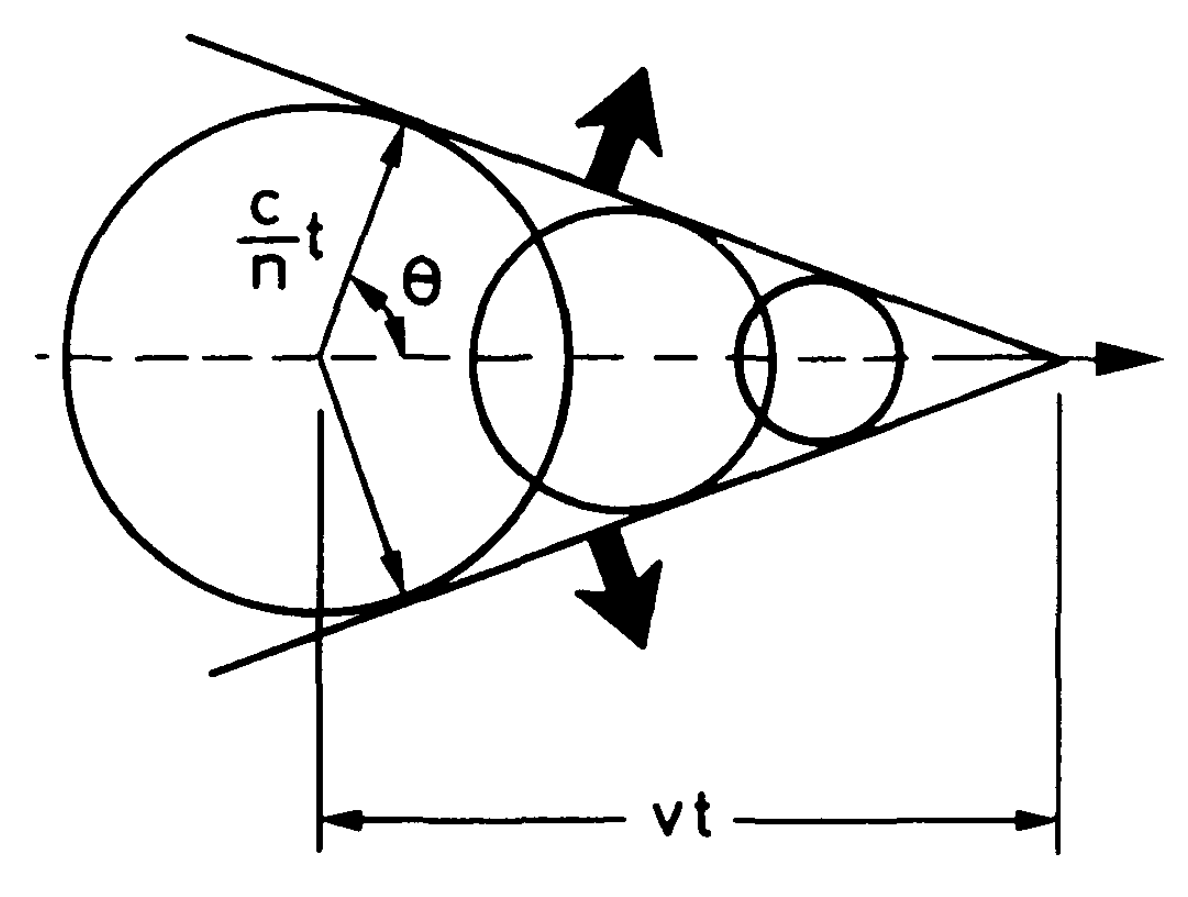
\includegraphics[width=6cm]{postextuais/apendice/figuras/cherenkov.png}
    \caption{Radiação de Cherenkov: uma onda de choque eletromagnética formada pela passagem de partículas acima da velocidade da luz no meio}
    \label{fig:my_label}
\end{figure}

em respeito à trajetória da partícula. A radiação incide em forma de fótons, geralmente no espectro do ultra-violeta, detectáveis por materiais fotosensíveis como PMTs ou \ac{SiPMs}.